\documentclass{minimal}
\usepackage{bm}
\usepackage{epsfig,color}
\usepackage[papersize={576.00bp,432.00bp},text={576.00bp,432.00bp}]{geometry}
\begin{document}
\centering
% Title: glps_renderer figure
% Creator: GL2PS 1.3.8, (C) 1999-2012 C. Geuzaine
% For: Octave
% CreationDate: Mon Aug 31 11:31:35 2015
\setlength{\unitlength}{1pt}
\begin{picture}(0,0)
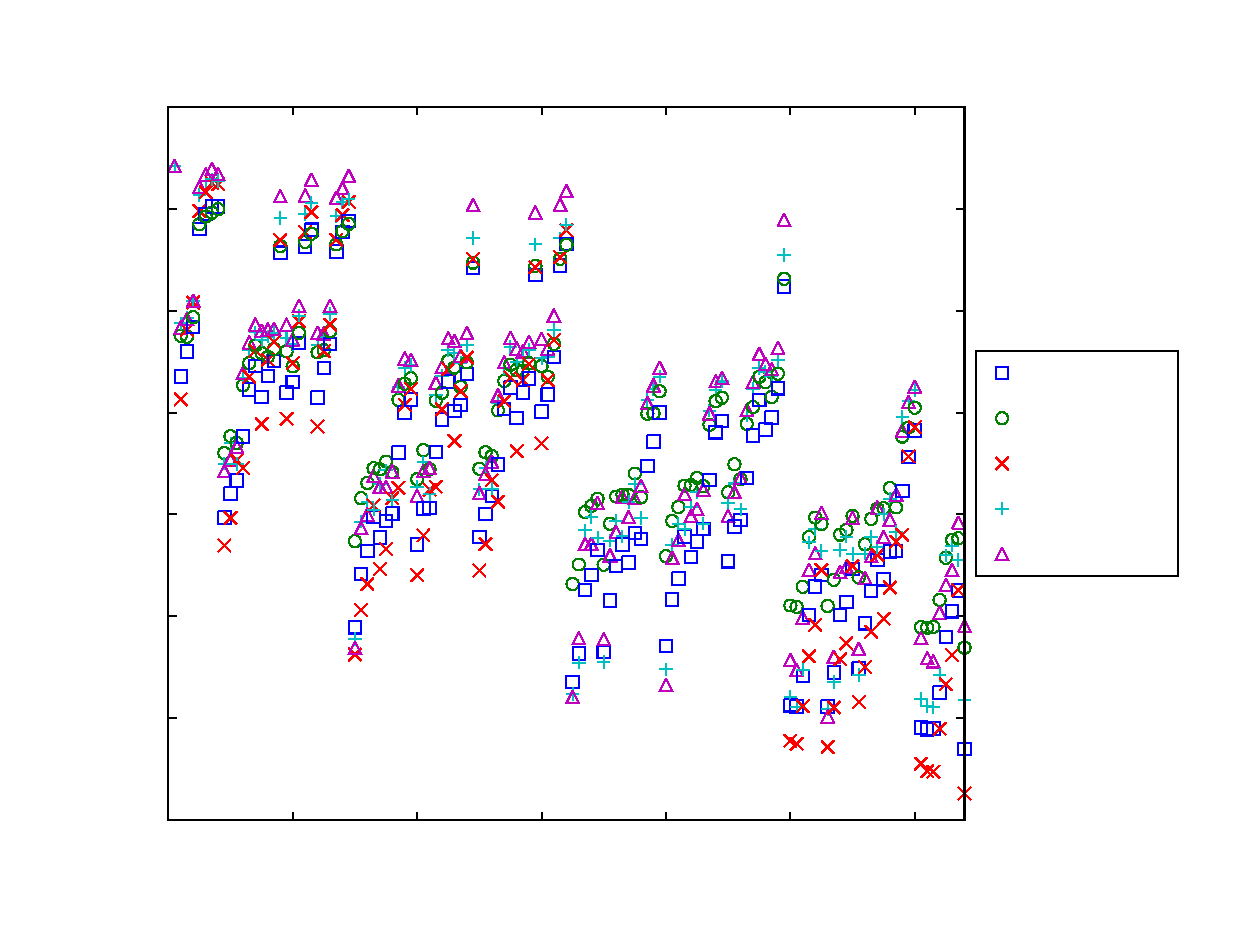
\includegraphics{dE_new-inc}
\end{picture}%
\begin{picture}(576,432)(0,0)
\fontsize{16}{0}
\selectfont\put(72.7998,41.1958){\makebox(0,0)[t]{\textcolor[rgb]{0,0,0}{{0}}}}
\fontsize{16}{0}
\selectfont\put(132.513,41.1958){\makebox(0,0)[t]{\textcolor[rgb]{0,0,0}{{20}}}}
\fontsize{16}{0}
\selectfont\put(192.226,41.1958){\makebox(0,0)[t]{\textcolor[rgb]{0,0,0}{{40}}}}
\fontsize{16}{0}
\selectfont\put(251.938,41.1958){\makebox(0,0)[t]{\textcolor[rgb]{0,0,0}{{60}}}}
\fontsize{16}{0}
\selectfont\put(311.651,41.1958){\makebox(0,0)[t]{\textcolor[rgb]{0,0,0}{{80}}}}
\fontsize{16}{0}
\selectfont\put(371.363,41.1958){\makebox(0,0)[t]{\textcolor[rgb]{0,0,0}{{100}}}}
\fontsize{16}{0}
\selectfont\put(431.076,41.1958){\makebox(0,0)[t]{\textcolor[rgb]{0,0,0}{{120}}}}
\fontsize{16}{0}
\selectfont\put(67.7979,46.2002){\makebox(0,0)[r]{\textcolor[rgb]{0,0,0}{{-14}}}}
\fontsize{16}{0}
\selectfont\put(67.7979,95.1001){\makebox(0,0)[r]{\textcolor[rgb]{0,0,0}{{-13}}}}
\fontsize{16}{0}
\selectfont\put(67.7979,144){\makebox(0,0)[r]{\textcolor[rgb]{0,0,0}{{-12}}}}
\fontsize{16}{0}
\selectfont\put(67.7979,192.9){\makebox(0,0)[r]{\textcolor[rgb]{0,0,0}{{-11}}}}
\fontsize{16}{0}
\selectfont\put(67.7979,241.8){\makebox(0,0)[r]{\textcolor[rgb]{0,0,0}{{-10}}}}
\fontsize{16}{0}
\selectfont\put(67.7979,290.7){\makebox(0,0)[r]{\textcolor[rgb]{0,0,0}{{-9}}}}
\fontsize{16}{0}
\selectfont\put(67.7979,339.6){\makebox(0,0)[r]{\textcolor[rgb]{0,0,0}{{-8}}}}
\fontsize{16}{0}
\selectfont\put(67.7979,388.5){\makebox(0,0)[r]{\textcolor[rgb]{0,0,0}{{-7}}}}
\fontsize{16}{0}
\selectfont\put(263.881,28.1958){\makebox(0,0)[t]{\textcolor[rgb]{0,0,0}{{\textbf{cluster}}}}}
\fontsize{16}{0}
\selectfont\put(47.7979,217.35){\rotatebox{90}{\makebox(0,0)[b]{\textcolor[rgb]{0,0,0}{{$E^+ - E^0$ [eV]}}}}}
\fontsize{16}{0}
\selectfont\put(485.661,260.689){\makebox(0,0)[l]{\textcolor[rgb]{0,0,0}{{gaussian}}}}
\fontsize{16}{0}
\selectfont\put(485.661,239.02){\makebox(0,0)[l]{\textcolor[rgb]{0,0,0}{{abinit}}}}
\fontsize{16}{0}
\selectfont\put(485.661,217.35){\makebox(0,0)[l]{\textcolor[rgb]{0,0,0}{{nwchem}}}}
\fontsize{16}{0}
\selectfont\put(485.661,195.681){\makebox(0,0)[l]{\textcolor[rgb]{0,0,0}{{NN (I)}}}}
\fontsize{16}{0}
\selectfont\put(485.661,174.011){\makebox(0,0)[l]{\textcolor[rgb]{0,0,0}{{NN (II)}}}}
\end{picture}
\end{document}
